\scanpage{48}
une \unsure{pure|vraie} variation modulaire de $X_0$, s'exprimant disons par le fait que $X_0$ est la fibre, en un point $t_0$ au dessus du pt fermé $s$ de $S$, d'un schéma propre et lisse \inserted{$Y$} sur un $M$ de type fini sur $S$.
\margin{\figure{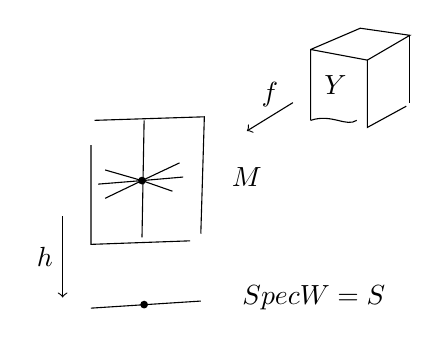
\begin{tikzpicture}[x=0.9cm,y=0.9cm]
\draw (3.5,3.3)--(3.5,4.3)--(4.2,4.6)--(4.9,4.5)--(4.3,4.15)--(3.5,4.3);
\draw (4.3,4.15)--(4.3,3.2)--(4.85,3.5);
\draw (4.9,4.5)--(4.9,3.55);
\draw (3.5,3.3)..controls(3.8,3.4)and(4.0,3.2)..(4.15,3.3);
\node at (3.85,3.8) {$Y$};
\draw[->] (3.25,3.55)--(2.6,3.15) node[midway,above] {$f$};
\draw (0.45,3.3)--(2.0,3.35)--(1.95,1.7);
\draw (0.4,2.95)--(0.4,1.55)--(1.8,1.6);
\draw (1.15,3.3)--(1.12,1.65);
\draw (0.6,2.6)--(1.12,2.45)--(1.65,2.7);
\draw (0.5,2.4)--(1.12,2.45)--(1.7,2.5);
\draw (0.6,2.2)--(1.12,2.45)--(1.55,2.3);
\fill (1.12,2.45) circle(1.4pt);
\node at (2.6,2.5) {$M$};
\draw[->] (0,1.95)--(0,0.8) node[midway,left] {$\unsure{h}$};
\draw (0.4,0.65)--(1.95,0.75);
\fill (1.15,0.7) circle(1.4pt);
\node[right] at (2.4,0.8) {$\operatorname{Spec}W=S$};
\end{tikzpicture}}}
Les différentes sections de $M$ sur $S$ donneront différentes façons de relever $X_0$ en un $X$ propre et lisse sur $S$. Prenant
\[
(*)\qquad K^\bullet=Rf_*(\underline{\Omega}^\bullet_{Y/M})
\]
on voit que pour \unsure{tte} telle section $g$ de $M$ sur $S$, définissant un $X_g^{\deleted{\unsure{g}}}$, et
\[
f_g^{\deleted{\unsure{g}}}:X_g^{\deleted{\unsure{g}}}\longrightarrow S
\]
\margin{$\unsure{\left(k+\frac12\right)\log(k+1)}
-\unsure{\left(k-\frac12\right)\log}$}
on a
\[
\mathbb{R}f_{g*}(\underline{\Omega}^*_{X_g/S})
\underset{\substack{\text{isom}\\\text{can}}}{\xleftarrow{\sim}}
g^*(K^\bullet)
\]
($g^*$ au sens des catégories dérivées ....). Il s'ensuit, \unsure{de même manière triviale}, que
\[
\mathbb{R}^if_{g*}(\underline{\Omega}^*_{X_g/S})
\xleftarrow{\sim}g^*(\mathcal{H}^i)
\]
\margin{47}
